% ==================================================
% Linearity and Operator Algebra
% Discrete Calculus --- Difference Operators
% ==================================================

\subsection{Properties of the Difference Operator}
\label{subsec:difference-operator-properties}

\begin{exposition}
The forward difference operator satisfies algebraic properties that
closely mirror the familiar rules of differentiation.
\end{exposition}

\subsection*{Linearity}

\begin{proposition}[Linearity of \(\Delta\)]
\label{prop:delta-linearity}
For functions \(f,g : \mathbb{Z} \to \mathbb{R}\) and constants \(a,b \in \mathbb{R}\),
\[
\Delta (a f + b g)
=
a\,\Delta f + b\,\Delta g.
\]
\hyperref[prf:delta-linearity]{\textit{Go to proof.}}
\end{proposition}

\begin{remark*}[Standard quantified statement]
\(\forall f,g : \mathbb{Z}\to\mathbb{R},\;
\forall a,b \in \mathbb{R},\;
\forall n \in \mathbb{Z}:\;
\Delta(af+bg)(n) = a\,\Delta f(n) + b\,\Delta g(n)\).
\end{remark*}

\begin{remark*}[Predicate reading]
\[
  \operatorname{LinearOperator}(\Delta)
  \;\colonequiv\;
  \forall f,g\,\forall a,b\,\forall n,\;
  \Delta(af+bg)(n)=a\,\Delta f(n)+b\,\Delta g(n).
\]
\end{remark*}

\begin{remark*}[Interpretation]
Taking a forward difference respects pointwise linear combinations.
\end{remark*}

\begin{dependencies}
\begin{itemize}
  \item \hyperref[def:forward-difference]{Forward Difference Operator}.
\end{itemize}
\end{dependencies}


\subsection*{Constant Rule}

\begin{proposition}[Constant rule]
\label{prop:delta-constant}
If \(c\) is a constant function, then \(\Delta c = 0\).
\hyperref[prf:delta-constant]{\textit{Go to proof.}}
\end{proposition}

\begin{remark*}[Standard quantified statement]
\(\forall c \in \mathbb{R},\; \forall n \in \mathbb{Z}:\; \Delta c(n) = 0\).
\end{remark*}

\begin{remark*}[Predicate reading]
\[
  \operatorname{ConstantRule}(\Delta)
  \;\colonequiv\;
  \forall c\in\mathbb R\,\forall n\in\mathbb Z,\; \Delta c(n)=0.
\]
\end{remark*}

\begin{remark*}[Interpretation]
A constant discrete function has no one-step change.
\end{remark*}

\begin{dependencies}
\begin{itemize}
  \item \hyperref[def:forward-difference]{Forward Difference Operator}.
\end{itemize}
\end{dependencies}


\begin{exposition}
This mirrors \(\tfrac{d}{dx} c = 0\) in continuous calculus.
\end{exposition}

\subsection*{The Shift Operator and Operator Algebra}

\begin{definition}[Shift Operator]
\label{def:shift-operator}
The \emph{shift operator} \(E\) and the \emph{identity operator} \(I\)
are defined by
\[
Ef(n) = f(n+1), \qquad If(n) = f(n).
\]
\end{definition}

\DefinitionalRoot

\begin{remark*}[Standard quantified statement]
\(\forall f : \mathbb{Z}\to\mathbb{R},\; \forall n \in \mathbb{Z}:\;
Ef(n) = f(n+1)\) and \(If(n) = f(n)\).
\end{remark*}

\begin{remark*}[Predicate reading]
\[
  S_E=\mathsf{ShiftOperator}(E,\mathbb Z)
  \;\colonequiv\;
  \forall f:\mathbb Z\to\mathbb R\,\forall n\in\mathbb Z,\;
  Ef(n)=f(n+1).
\]
\end{remark*}

\begin{remark*}[Interpretation]
The shift operator advances the input by one step, while the identity
operator leaves the input unchanged.
\end{remark*}

\begin{theorem}[\(\Delta = E - I\)]
\label{thm:delta-shift-minus-identity}
\[
\Delta = E - I.
\]
\hyperref[prf:delta-shift-minus-identity]{\textit{Go to proof.}}
\end{theorem}

\begin{remark*}[Standard quantified statement]
\(\forall f : \mathbb{Z}\to\mathbb{R},\; \forall n \in \mathbb{Z}:\;
\Delta f(n) = (E-I)f(n) = f(n+1) - f(n)\).
\end{remark*}

\begin{remark*}[Predicate reading]
\[
  \operatorname{OperatorIdentity}(\Delta,E-I)
  \;\colonequiv\;
  \forall f\,\forall n,\; \Delta f(n)=(E-I)f(n).
\]
\end{remark*}

\begin{remark*}[Interpretation]
The forward difference is the s
hifted value minus the original value.
\end{remark*}

\begin{dependencies}
\begin{itemize}
  \item \hyperref[def:forward-difference]{Forward Difference Operator}.
  \item \hyperref[def:shift-operator]{Shift Operator}.
\end{itemize}
\end{dependencies}


\begin{exposition}
Expressing \(\Delta = E - I\) reveals that higher differences can be
computed using ordinary algebra. Applying the binomial theorem to
\(\Delta^n = (E-I)^n\) gives
\[
\Delta^n
=
\sum_{k=0}^{n}
(-1)^{\,n-k}
\binom{n}{k}
E^{k}.
\]
Since \(E^k f(n) = f(n+k)\), this yields
\[
\Delta^n f(n)
=
\sum_{k=0}^{n}
(-1)^{\,n-k}
\binom{n}{k}
f(n+k).
\]
This explains why binomial coefficients and Pascal's triangle appear
naturally throughout discrete calculus: they are a direct consequence
of the algebraic identity \(\Delta = E - I\).
\end{exposition}

\subsection{Difference Tables and Polynomial Detection}
\label{subsec:difference-tables}

\begin{exposition}
One of the most useful tools in discrete calculus is the \emph{difference
table}. By repeatedly applying the difference operator to a sequence,
one can detect whether the sequence arises from a polynomial function and
determine its degree.
\end{exposition}

\begin{definition}[Difference Table]
\label{def:difference-table}
Given a sequence \(f(0), f(1), f(2), \dots\), the \emph{difference table}
is constructed by listing the successive values of the function and then
computing their forward differences \(\Delta f(n) = f(n+1)-f(n)\),
then \(\Delta^2 f\), \(\Delta^3 f\), and so on.
\end{definition}

\begin{remark*}[Standard quantified statement]
\[
\Delta^0 f=f,\qquad
\Delta^{k+1}f=\Delta(\Delta^k f)\quad(k\ge 0).
\]
\end{remark*}

\begin{remark*}[Interpretation]
A difference table organizes repeated forward differences into rows so that
eventual constant or zero rows become visible.
\end{remark*}

\begin{dependencies}
\begin{itemize}
  \item \hyperref[def:forward-difference]{Forward Difference Operator}.
  \item \hyperref[def:higher-differences]{Higher Differences}.
\end{itemize}
\end{dependencies}

\subsection*{Example}

\begin{example*}
For \(f(n) = n^2\):

\[
\begin{array}{c|c|c|c}
n & f(n) & \Delta f(n) & \Delta^2 f(n) \\
\hline
0 & 0  & 1 &   \\
1 & 1  & 3 & 2 \\
2 & 4  & 5 & 2 \\
3 & 9  & 7 & 2 \\
4 & 16 & 9 & 2 \\
5 & 25 &   &
\end{array}
\]

The second differences are constant (all equal to \(2\)), and the third
differences are zero.
\end{example*}

\begin{center}
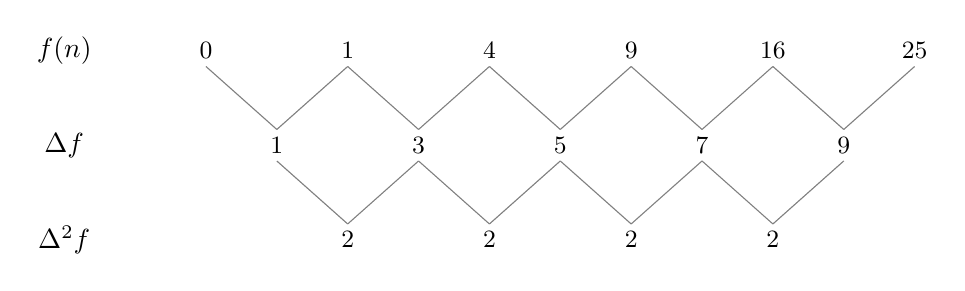
\begin{tikzpicture}[
    every node/.style={font=\small},
    lbl/.style={font=\bfseries}
]
\node[lbl] at (-1.8, 0) {$f(n)$};
\node[lbl] at (-1.8,-1.2) {$\Delta f$};
\node[lbl] at (-1.8,-2.4) {$\Delta^2 f$};

\node at (0,0) {$0$}; \node at (1.8,0) {$1$};
\node at (3.6,0) {$4$}; \node at (5.4,0) {$9$};
\node at (7.2,0) {$16$}; \node at (9.0,0) {$25$};

\node at (0.9,-1.2) {$1$}; \node at (2.7,-1.2) {$3$};
\node at (4.5,-1.2) {$5$}; \node at (6.3,-1.2) {$7$};
\node at (8.1,-1.2) {$9$};

\node at (1.8,-2.4) {$2$}; \node at (3.6,-2.4) {$2$};
\node at (5.4,-2.4) {$2$}; \node at (7.2,-2.4) {$2$};

\draw[gray] (0,-0.2) -- (0.9,-1.0); \draw[gray] (1.8,-0.2) -- (0.9,-1.0);
\draw[gray] (1.8,-0.2) -- (2.7,-1.0); \draw[gray] (3.6,-0.2) -- (2.7,-1.0);
\draw[gray] (3.6,-0.2) -- (4.5,-1.0); \draw[gray] (5.4,-0.2) -- (4.5,-1.0);
\draw[gray] (5.4,-0.2) -- (6.3,-1.0); \draw[gray] (7.2,-0.2) -- (6.3,-1.0);
\draw[gray] (7.2,-0.2) -- (8.1,-1.0); \draw[gray] (9.0,-0.2) -- (8.1,-1.0);

\draw[gray] (0.9,-1.4) -- (1.8,-2.2); \draw[gray] (2.7,-1.4) -- (1.8,-2.2);
\draw[gray] (2.7,-1.4) -- (3.6,-2.2); \draw[gray] (4.5,-1.4) -- (3.6,-2.2);
\draw[gray] (4.5,-1.4) -- (5.4,-2.2); \draw[gray] (6.3,-1.4) -- (5.4,-2.2);
\draw[gray] (6.3,-1.4) -- (7.2,-2.2); \draw[gray] (8.1,-1.4) -- (7.2,-2.2);
\end{tikzpicture}

\end{center}

\begin{theorem}[Polynomial detection]
\label{thm:polynomial-detection}
Let \(f(n)\) be a sequence generated by a polynomial of degree \(d\). Then
\(\Delta^d f(n)\) is constant, and \(\Delta^{d+1} f(n) = 0\).
\hyperref[prf:polynomial-detection]{\textit{Go to proof.}}
\end{theorem}


\begin{remark*}[Standard quantified statement]
\(\forall d \in \mathbb{N},\; \forall f : \mathbb{Z}\to\mathbb{R}\) polynomial of degree \(d\):\\
\(\exists c \in \mathbb{R}: \forall n \in \mathbb{Z},\; \Delta^d f(n) = c\),
and \(\forall n \in \mathbb{Z},\; \Delta^{d+1}f(n) = 0\).
\end{remark*}

\begin{remark*}[Predicate reading]
\[
  \operatorname{PolynomialDetection}(f,d)
  \;\colonequiv\;
  \operatorname{PolynomialDegree}(f,d)
  \Rightarrow
  \left(
    \exists c\,\forall n,\; \Delta^d f(n)=c
  \right)
  \wedge
  \forall n,\; \Delta^{d+1}f(n)=0.
\]
\end{remark*}

\begin{remark*}[Interpretation]
Repeated differences reveal polynomial degree: a degree \(d\) polynomial has
constant \(d\)-th differences and vanishing next differences.


Difference tables provide a practical method for identifying polynomial
sequences and determining their degree. This observation leads naturally to
the \emph{falling factorial basis}: a family of polynomials that interact
particularly cleanly with the difference operator, forming the foundation
for Newton's discrete analogue of the Taylor expansion.
\end{remark*}

\begin{dependencies}
\begin{itemize}
  \item \hyperref[def:forward-difference]{Forward Difference Operator}.
  \item \hyperref[def:higher-differences]{Higher Differences}.
  \item \hyperref[def:difference-table]{Difference Table}.
  \item \hyperref[thm:binomial-theorem]{Binomial Theorem}.
\end{itemize}
\end{dependencies}
